\section{Design Objectives and Development Process}
\label{sec:gear-design-construction}

GEAR relies on a common representation of agentic systems that is independent
of the APIs and execution mechanisms of individual frameworks. Constructing
this representation required identifying the relevant domain concepts,
organizing their variability, and determining how they can be implemented in
different target frameworks.

This process followed three design objectives: making the configuration space
of agentic systems explicit, separating system specifications from
framework-specific implementations, and supporting the automated and
reproducible generation of executable systems. We first analyze the scientific
literature and select the frameworks considered in this work. We then derive
the common variability model, define its mappings to the target frameworks,
and iteratively validate the resulting models and mappings.


\subsection{Design Objectives}
\label{subsec:design-objectives}

The three objectives introduced above translate the motivations of GEAR into
development requirements. First, the relevant configuration decisions and
their constraints must be represented explicitly. Second, this representation
must remain independent of framework APIs and implementation mechanisms.
Third, a valid specification must be transformable into reproducible,
executable artifacts for a selected target framework.

To operationalize these objectives, we first analyzed the scientific
literature to identify the dimensions used to characterize \gls{llm}-based
agents and \gls{mas}s. This analysis established the functional boundary of
the common representation before any framework artifact was inspected.

\paragraph{\textbf{Functional scope derived from the literature.}}
Existing studies describe \gls{llm}-based agents through characteristics such
as their profiles, goals, reasoning, planning, memory, actions, tools,
perception, and interactions with their environment
~\cite{xi2025rise,guo2024large}. At the multi-agent level, additional
characteristics concern communication, coordination, topology, orchestration,
and capability acquisition. \etal{Wu}~\cite{wu2024autogen} also emphasize agent
configuration, human participation, tool use, and programmable interaction
patterns.

The organization and behaviour of an \gls{mas} further depend on its
orchestration logic, communication mechanisms, memory management, control flow,
and error-handling strategies~\cite{emde2026maseval}. Finally, traces, logs,
metrics, and execution events provide mechanisms for observing the system at
runtime~\cite{dong2024agentops}.

Based on this analysis, we delimited the functional scope considered in this
work. We retained the categories that directly concern the configuration,
composition, and execution of orchestrated software agents. Other dimensions
identified in the literature remain relevant to agentic systems, but require
distinct models and evaluation protocols. They were therefore excluded from
the current scope, as reported in
Table~\ref{tab:functional-scope}.

\begin{table*}[t]
    \centering
    \caption{Functional categories identified from the literature and their
    inclusion in the scope of the study.}
    \label{tab:functional-scope}
    \small
    \begin{tabularx}{\textwidth}{
        @{}
        p{0.17\textwidth}
        >{\raggedright\arraybackslash}X
        >{\centering\arraybackslash}p{0.09\textwidth}
        p{0.29\textwidth}
        @{}
    }
        \toprule
        \textbf{Category}
        & \textbf{Considered characteristics}
        & \textbf{Included}
        & \textbf{Scope rationale} \\
        \midrule

        Agent specification
        & Identity, role, goals, instructions, capabilities, and
        contextual description
        & \(\checkmark\)
        & These elements define the responsibilities and expected
        behaviour of each agent. \\

        Model configuration
        & Model, provider, endpoint, generation parameters, timeout, and
        retry parameters
        & \(\checkmark\)
        & These configuration decisions can affect agent behaviour and
        execution across frameworks. \\

        Tasks and planning
        & Task descriptions, objectives, inputs, expected outputs,
        decomposition, and dependencies
        & \(\checkmark\)
        & Tasks constitute configurable units of work and define how the
        system objectives are operationalized. \\

        Tools
        & Tool declarations, tool schemas, association with agents, and
        tool invocation
        & \(\checkmark\)
        & Tools determine how agents act on external resources and extend
        their capabilities. \\

        Memory and state
        & Individual memory, shared memory, workflow state, and propagation of
        intermediate results
        & \(\checkmark\)
        & Memory and state determine how information is retained and
        shared during execution. \\

        Data and outputs
        & Textual outputs, JSON outputs, typed models, schemas, and output
        validation
        & \(\checkmark\)
        & Output contracts determine how information is exchanged between
        tasks, agents, and external components. \\

        Orchestration and topology
        & Sequential and parallel execution, delegation, handoffs,
        fan-out/fan-in, aggregation, nodes, edges, and dependencies
        & \(\checkmark\)
        & These characteristics define the structural organization and
        coordination of the system. \\

        Control flow
        & Conditions, branches, loops, routing decisions, and termination
        conditions
        & \(\checkmark\)
        & Control-flow mechanisms determine which components are executed
        and under which conditions. \\

        Execution properties
        & Synchronous and asynchronous execution, execution limits,
        retries, error handling, caching, and human intervention
        & \(\checkmark\)
        & These properties influence the runtime semantics and robustness
        of the generated system. \\

        \midrule

        Communication protocols
        & Explicit messages, message types, communication channels,
        conversation protocols, and negotiation mechanisms
        & \(\times\)
        & Communication is a central multi-agent dimension, but comparing
        protocol semantics would require a separate interaction-level
        analysis. \\

        Perception and environment
        & Sensor modalities, perception pipelines, environment models, and
        environment-specific actions
        & \(\times\)
        & The study focuses on orchestrated software agents rather than
        embodied agents or domain-specific perception mechanisms. \\

        Learning and evolution
        & Online learning, self-improvement, capability acquisition, and
        runtime evolution
        & \(\times\)
        & The study evaluates system configuration and execution, not
        model training or agent-learning processes. \\

        Observability
        & Traces, logs, metrics, monitoring, runtime events, and execution
        analytics
        & \(\times\)
        & Observability concerns the operational analysis of executions
        and is evaluated separately from functional coverage. \\

        Security and governance
        & Identities, permissions, access control, isolation, policies, and
        audit mechanisms
        & \(\times\)
        & These mechanisms require a dedicated security model, threat
        analysis, and evaluation protocol. \\

        \bottomrule
    \end{tabularx}
\end{table*}

This delimitation was established before the framework artifact analysis. The
nine included categories define the analysis grid used to extract and compare
framework concepts during the subsequent artifact analysis. At this stage,
they remain domain categories rather than features of the GEAR model and do
not indicate whether a capability is supported by a particular framework.

\subsection{Selection of the Studied Frameworks}
\label{subsec:literature-framework-selection}

\paragraph{\textbf{Identification of candidate frameworks.}}
Candidate frameworks were identified from recent scientific studies on
\gls{llm}-based agents and \gls{mas}s. We extended this initial set by examining
official documentation and public source-code repositories related to agent
development, multi-agent orchestration, and agent workflow construction.
Frameworks and alternatives referenced by these sources were also considered.

The identification process covered projects presented as agent frameworks,
multi-agent frameworks, orchestration frameworks, workflow frameworks, or agent
development kits. Duplicate entries, renamed projects, and projects replaced by
a maintained successor were consolidated under their current implementation.

The objective was not to establish an exhaustive inventory of agent
technologies, but to obtain a sufficiently diverse set of candidates. The
complete list of candidates and their screening decisions is reported in
Appendix~\ref{appendix:candidate-frameworks}. The identification and selection
process was completed in July 2026.

\paragraph{\textbf{Framework selection.}}
A candidate was eligible when it was publicly accessible, sufficiently
documented, actively maintained, and available through an identifiable and
installable version. It also had to provide a Python API, support the definition
of \gls{llm}-based agents, and enable the composition of multiple agents, tasks,
or workflow components.

We excluded libraries limited to direct \gls{llm} calls, closed platforms
without an accessible API, inactive projects, observability tools without
agent-construction capabilities, frameworks dedicated exclusively to
reinforcement-learning agents, and frameworks supporting only languages other
than Python.

Among the eligible candidates, we selected frameworks representing
complementary approaches to agent definition, task specification, model and
tool integration, memory and state management, data and outputs, orchestration,
control flow, and execution. This process resulted in the ten frameworks
presented in Table~\ref{tab:framework-metadata}. For reproducibility, the table
reports the reference version targeted by GEAR, its release date, and a link to
the official documentation.

\begin{table*}[t]
    \centering
    \caption{Metadata documenting the selection of the studied frameworks.
    The versions correspond to the reference versions targeted by GEAR.}
    \label{tab:framework-metadata}
    \small
    \begin{tabular}{
        @{}
        p{0.18\textwidth}
        p{0.08\textwidth}
        p{0.10\textwidth}
        p{0.17\textwidth}
        p{0.32\textwidth}
        @{}
    }
        \toprule
        \textbf{Framework}
        & \textbf{Version}
        & \textbf{Release date}
        & \textbf{Official source}
        & \textbf{Reason for inclusion} \\
        \midrule

        CrewAI
        & 1.15.4
        & 2026-07-17
        & \href{https://docs.crewai.com/}{Documentation}
        & Role- and task-based orchestration \\

        Google ADK
        & 2.5.0
        & 2026-07-16
        & \href{https://adk.dev/}{Documentation}
        & Hierarchical agents and graph-based workflow agents \\

        LangGraph
        & 1.0.0
        & 2025-10-17
        & \href{https://docs.langchain.com/oss/python/langgraph/overview}
        {Documentation}
        & Stateful graph-based workflows with branching and joins \\

        OpenAI Agents SDK
        & 0.18.0
        & 2026-07-07
        & \href{https://openai.github.io/openai-agents-python/}
        {Documentation}
        & Agent handoffs and native tracing capabilities \\

        Microsoft Agent Framework
        & 1.11.0
        & 2026-07-10
        & \href{https://learn.microsoft.com/en-us/agent-framework/}
        {Documentation}
        & Enterprise agent workflows with fan-out and synchronized fan-in
        orchestration \\

        Strands Agents
        & 1.48.0
        & 2026-07-17
        & \href{https://strandsagents.com/docs/}
        {Documentation}
        & Lightweight composition of deterministic multi-agent graphs \\

        PydanticAI
        & 2.13.0
        & 2026-07-18
        & \href{https://pydantic.dev/docs/ai/overview/}
        {Documentation}
        & Type-safe agents and structured outputs \\

        AutoGen
        & 0.7.5
        & 2025-09-30
        & \href{https://microsoft.github.io/autogen/stable/user-guide/agentchat-user-guide/index.html}
        {Documentation}
        & Conversational agents and bounded agent teams \\

        Semantic Kernel
        & 1.44.0
        & 2026-07-07
        & \href{https://learn.microsoft.com/en-us/semantic-kernel/frameworks/agent/}
        {Documentation}
        & Service- and plugin-oriented agent architecture \\

        Haystack
        & 2.31.0
        & 2026-07-08
        & \href{https://docs.haystack.deepset.ai/docs/intro}
        {Documentation}
        & Pipeline-oriented agent and component composition \\

        \bottomrule
    \end{tabular}
\end{table*}

\subsection{Analysis of Framework Artifacts}
\label{subsec:framework-artifact-analysis}

After selecting the ten frameworks, we analyzed their artifacts to refine the
domain concepts identified from the literature. The objective of this stage was
to construct a traceable inventory of configuration elements before deciding
how they should be normalized in the common variability model.


\paragraph{\textbf{Framework artifact analysis and concept extraction.}}
For each framework, we analyzed the official documentation, API references,
configuration mechanisms, and implementation examples. Public source code was
consulted when these sources did not sufficiently clarify the semantics or
dependencies of a configuration option.

The functional categories retained in Table~\ref{tab:functional-scope} were used
as the analysis grid. For each identified element, we recorded its
framework-specific name, its semantics, the entity to which it applies, its
possible values, and its relationships with other elements. The extracted
elements were then classified into the four types presented in
Table~\ref{tab:extracted-element-types}.

\begin{table*}[t]
    \centering
    \caption{Types of elements extracted from the selected frameworks.}
    \label{tab:extracted-element-types}
    \footnotesize
    \begin{tabularx}{\textwidth}{
        @{}
        p{0.18\textwidth}
        >{\raggedright\arraybackslash}X
        p{0.31\textwidth}
        @{}
    }
        \toprule
        \textbf{Element type}
        & \textbf{Description}
        & \textbf{Examples} \\
        \midrule

        Domain concept
        & Principal entity involved in the specification or execution of an
        agentic system
        & Agent, task, model, tool, module, workflow \\

        Capability
        & Behaviour or functionality that can be assigned to a domain concept
        & Memory, reasoning, delegation, human intervention \\

        Variation point
        & Configuration decision admitting several values, alternatives, or
        implementations
        & Model provider, execution strategy, output format, retry policy \\

        Constraint
        & Dependency, incompatibility, or condition governing the selection of
        configuration options
        & Required credentials, incompatible providers, conditional parameters \\

        \bottomrule
    \end{tabularx}
\end{table*}

A concept did not need to be supported by all ten frameworks to be retained.
It was included when it represented a meaningful configuration decision for
\gls{llm}-based \gls{mas}s and could be expressed independently of a particular
framework. Constructs whose semantics could not be generalized were kept as
framework-specific implementation details.

\subsection{Derivation of the Common Variability Model}
\label{subsec:common-variability-model}

The common variability model was derived from the extracted inventory rather
than from the terminology of any single framework. The derivation comprised
three steps: normalization and consolidation of the extracted elements,
organization of the resulting concepts into feature models, and definition of
their relations and constraints.

\paragraph{\textbf{Normalization and consolidation.}}
The extracted elements were compared according to their semantics rather than
their names. Elements expressing the same configuration decision were
consolidated under a common concept. For example, constructs used to provide
instructions, system prompts, or contextual descriptions were associated with
a common agent configuration concern when they played an equivalent role.

Conversely, similarly named elements were kept separate when they produced
different behaviours. For each element, we therefore considered its purpose,
its effect on the system, its relationships with other elements, and whether
its semantics could be preserved across frameworks. Common decisions became
features, while their possible implementations were represented as
subfeatures or configurable values. This process produced the
framework-independent vocabulary used by GEAR.


\paragraph{\textbf{Construction of the feature models.}}
The consolidated concepts were organized into three complementary feature
models: \texttt{GearAgent}, \texttt{GearModule}, and
\texttt{GearWorkflow}. Their scope and current characteristics are summarized
in Table~\ref{tab:gear-feature-models}.

\texttt{GearAgent} represents the configuration of an individual agent,
including its identity, model, task, tools, memory, reasoning mechanisms, and
execution controls. \texttt{GearModule} represents reusable orchestration
structures. It currently supports parallel modules, with an optional
aggregator, and loop modules, with an optional stopping condition.
\texttt{GearWorkflow} represents the system-level composition of agents and
modules, together with optional shared memory.

\begin{table*}[t]
    \centering
    \caption{Characteristics of the GEAR feature models.}
    \label{tab:gear-feature-models}
    \footnotesize
    \begin{tabularx}{\textwidth}{
        @{}
        p{0.13\textwidth}
        >{\raggedright\arraybackslash}X
        p{0.20\textwidth}
        r
        r
        r
        @{}
    }
        \toprule
        \textbf{Model}
        & \textbf{Configuration scope}
        & \textbf{UVL artifact}
        & \textbf{Features}
        & \textbf{Constraints}
        & \textbf{Valid configurations} \\
        \midrule

        \texttt{GearAgent}
        & Definition and execution of an individual agent
        & \texttt{gear-agent.uvl}
        & 41
        & 9
        & \(10\,485\,760\) \\

        \texttt{GearModule}
        & Reusable parallel and loop orchestration structures
        & \texttt{gear-module.uvl}
        & 10
        & 0
        & 4 \\

        \texttt{GearWorkflow}
        & System-level composition of agents and modules
        & \texttt{gear-multiagent.uvl}
        & 6
        & 0
        & 4 \\

        \midrule
        \textbf{Total}
        & ---
        & ---
        & \textbf{57}
        & \textbf{9}
        & \textbf{51217928} \\

        \bottomrule
    \end{tabularx}

    \vspace{0.3em}
    \begin{minipage}{0.98\textwidth}
        \footnotesize
        The number of valid configurations is computed independently for each
        feature model. These values are not summed because agent and module
        models may be instantiated multiple times within a workflow.
    \end{minipage}
\end{table*}

Figure~\ref{fig:gear-feature-models} presents the three resulting feature
models. Their complete UVL representations are also available in the GEAR
repository described in Section~\ref{data}.

\begin{figure*}[t]
    \centering

    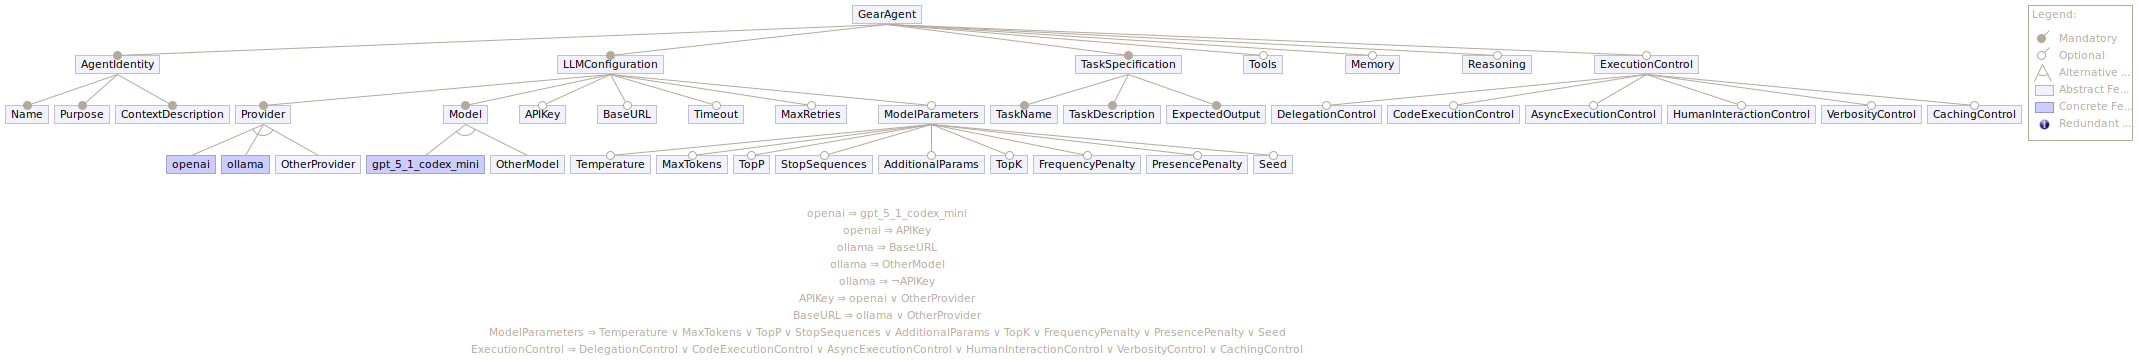
\includegraphics[width=\textwidth]
    {Figures/agent.png}

    \vspace{0.5em}

    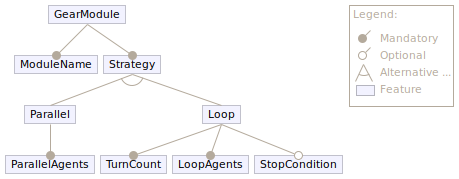
\includegraphics[width=0.48\textwidth]
    {Figures/module.png}
    \hfill
    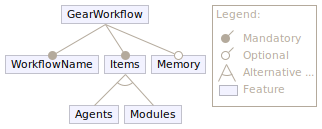
\includegraphics[width=0.48\textwidth]
    {Figures/workflow.png}

    \caption{GEAR feature models: \texttt{GearAgent} (top),
    \texttt{GearModule} (bottom left), and \texttt{GearWorkflow}
    (bottom right).}
    \label{fig:gear-feature-models}
\end{figure*}


\paragraph{\textbf{Definition and verification of constraints.}}
The features were connected through mandatory, optional, and alternative
relations. Mandatory relations represent elements required to define a valid
instance of their parent, while optional relations represent capabilities that
may be enabled depending on the intended system. Alternative groups represent
mutually exclusive configuration choices.

Cross-tree constraints were added when the hierarchy alone could not express a
dependency. For example, selecting the OpenAI provider requires an API key,
whereas selecting Ollama requires a base URL and excludes the OpenAI API key.
Similarly, selecting model parameters or execution controls requires at least
one corresponding subfeature.

The models and their constraints were expressed in the Universal Variability
Language (UVL). Framework-specific mechanisms that could not be generalized
were left to the mappings and connectors presented in the next subsection.

The resulting feature models constitute the common variability representation
used by GEAR. They separate the framework-independent specification of an
agentic system from the mechanisms required to instantiate it in a target
framework.

\subsection{Definition of Framework-Specific Mappings}
\label{subsec:mapping-target-frameworks}

The common variability model describes agents, modules, and workflows
independently of a particular framework. However, frameworks expose these
concepts through different APIs, properties, and execution mechanisms. A common
configuration decision may therefore have a direct representation in one
framework, require an adaptation in another, or remain unsupported.

GEAR addresses these differences through explicit mappings between the common
model and each supported target framework. These mappings separate the
description of the agentic system from the technical mechanisms used to
implement it.


\paragraph{\textbf{Identification of correspondences.}}
For each target framework, we examined how the concepts represented in
\texttt{GearAgent}, \texttt{GearModule}, and \texttt{GearWorkflow} can be
implemented using its public abstractions. At the agent level, this analysis
covered identity, models, instructions, tasks, tools, memory, reasoning, and
execution controls. At the module and workflow levels, it covered agent
composition, parallel and iterative execution, dependencies, and shared memory.

This step differs from the analysis performed during the derivation of the
common model. The previous step identified configuration concepts that are
relevant across frameworks. The present step determines how each concept can be
represented in a specific target framework.

For example, a parallel module may be implemented through a native parallel
agent, concurrent graph branches, or asynchronous execution primitives. These
mechanisms differ across frameworks but can represent the same orchestration
decision when they preserve the concurrent execution of the configured
elements.


\paragraph{\textbf{Definition of declarative mappings.}}
The identified correspondences were encoded in declarative YAML files. Separate
mappings describe agent, module, and workflow properties. Each entry identifies
a property from the common representation, its target abstraction, and the
nature of their correspondence.

A mapping entry follows the general structure:

\begin{verbatim}
- from: AgentIdentity.Name
  to: Agent.Name
  kind: direct
\end{verbatim}

The \texttt{from} field refers to a property in the common GEAR representation,
while the \texttt{to} field identifies its representation in the target
framework. Table~\ref{tab:mapping-types} presents the four correspondence types
used by GEAR.

\begin{table}[t]
    \centering
    \caption{Correspondence types used in framework mappings.}
    \label{tab:mapping-types}
    \footnotesize
    \begin{tabularx}{\columnwidth}{
        @{}
        p{0.23\columnwidth}
        >{\raggedright\arraybackslash}X
        @{}
    }
        \toprule
        \textbf{Type}
        & \textbf{Meaning} \\
        \midrule

        \texttt{direct}
        & The value can be transferred to a target property without changing
        its semantics. \\

        \texttt{equivalent}
        & The target uses a different abstraction that preserves the intended
        semantics. \\

        \texttt{partial}
        & The target represents only part of the common property or requires
        an explicit adaptation. \\

        \texttt{not\_mapped}
        & No sufficiently faithful target representation is available. \\

        \bottomrule
    \end{tabularx}
\end{table}

These mappings remain separate from the code-generation logic. They make the
correspondences inspectable and allow the support for a framework to evolve
without duplicating or modifying the common variability model.


\paragraph{\textbf{Treatment of semantic differences.}}
A valid GEAR configuration is not necessarily fully supported by every target
framework. When a framework provides a compatible abstraction, the selected
property is transferred directly or through an equivalent representation. When
only part of its semantics can be preserved, the mapping is declared as partial
and the required adaptation is handled during generation.

For example, a loop module may define both a maximum number of iterations and a
natural-language stopping condition. A target framework may support the
iteration limit without providing an executable representation of the stopping
condition. In this case, GEAR can map the iteration limit while explicitly
identifying the stopping condition as partially supported or unmapped.

The same issue occurs when a common property does not contain enough information
to construct the corresponding target element. A tool name, for instance, may
be insufficient when the framework also requires a callable implementation,
input schema, or dependency. GEAR does not generate such missing information
implicitly.

These distinctions prevent an incomplete translation from being considered
semantically exact. They also preserve traceability between the selected
features and their representation in the target framework. The mappings
therefore define the boundary between the common variability model and the
framework-specific generation mechanisms presented in
Section~\ref{subsec:gear-architecture-generation}.

\subsection{Iterative Validation and Refinement}
\label{subsec:iterative-validation-refinement}

The feature models, constraints, and framework-specific mappings were validated
iteratively against the artifacts of the ten selected frameworks. Missing
domain concepts were added, features were refined when their scope was too
general, and constraints were introduced when the comparison revealed
additional dependencies or incompatible choices.

The mappings were refined in the same loop. Implementing and exercising a
connector could reveal that a presumed direct correspondence required an
adaptation, that a target abstraction preserved only part of the intended
semantics, or that additional configuration information was required. The
correspondence type and the associated diagnostics were then updated
accordingly.

The process stopped when the common models covered the retained domain
concepts, their constraints admitted only structurally valid configurations,
and each selected feature had an explicit direct, equivalent, partial, or
unmapped status for every target framework. This iterative procedure separates
the construction and validation of the common representation from the tool
architecture that operationalizes it.

\section{The GEAR Tool}
\label{sec:gear-tool}
\label{subsec:gear-architecture-generation}

\subsection{Tool Overview and User Workflow}
\label{subsec:tool-overview-workflow}

GEAR implements the variability models and framework mappings through a
connector-based generation architecture. Its core components remain independent
of the target frameworks, while connectors encapsulate the information and
generation mechanisms required by each framework.

This separation enables the same GEAR configuration to be processed for
different targets without modifying the common variability model. It also
isolates framework-specific dependencies, templates, and adaptations from the
rest of the generation process.

From a user perspective, a GEAR workflow starts with the configuration of
agents, reusable modules, and their top-level composition. The user then selects
a target framework and requests generation. GEAR validates the configuration,
applies the corresponding mappings, produces the target project, and returns
the generated artifacts together with a conversion report.

\subsection{Tool Architecture}
\label{subsec:tool-architecture}

\paragraph{\textbf{Architecture overview.}}
Figure~\ref{fig:gear-architecture} presents the architecture of GEAR. The
configuration layer exposes the features defined by \texttt{GearAgent},
\texttt{GearModule}, and \texttt{GearWorkflow}. A selected configuration is
validated against these models before being transferred to the generation core.

The generation core interprets the selected features and constructs a
framework-independent intermediate representation of the configured system.
This representation describes the agents, modules, workflow structure,
properties, and relationships required for generation without relying on the
classes or syntax of a particular framework.

The connector corresponding to the selected target framework then translates
this representation into executable artifacts. It uses the mappings introduced
in Section~\ref{subsec:mapping-target-frameworks}, together with
framework-specific templates and assembly logic.

\begin{figure*}[t]
    \centering
    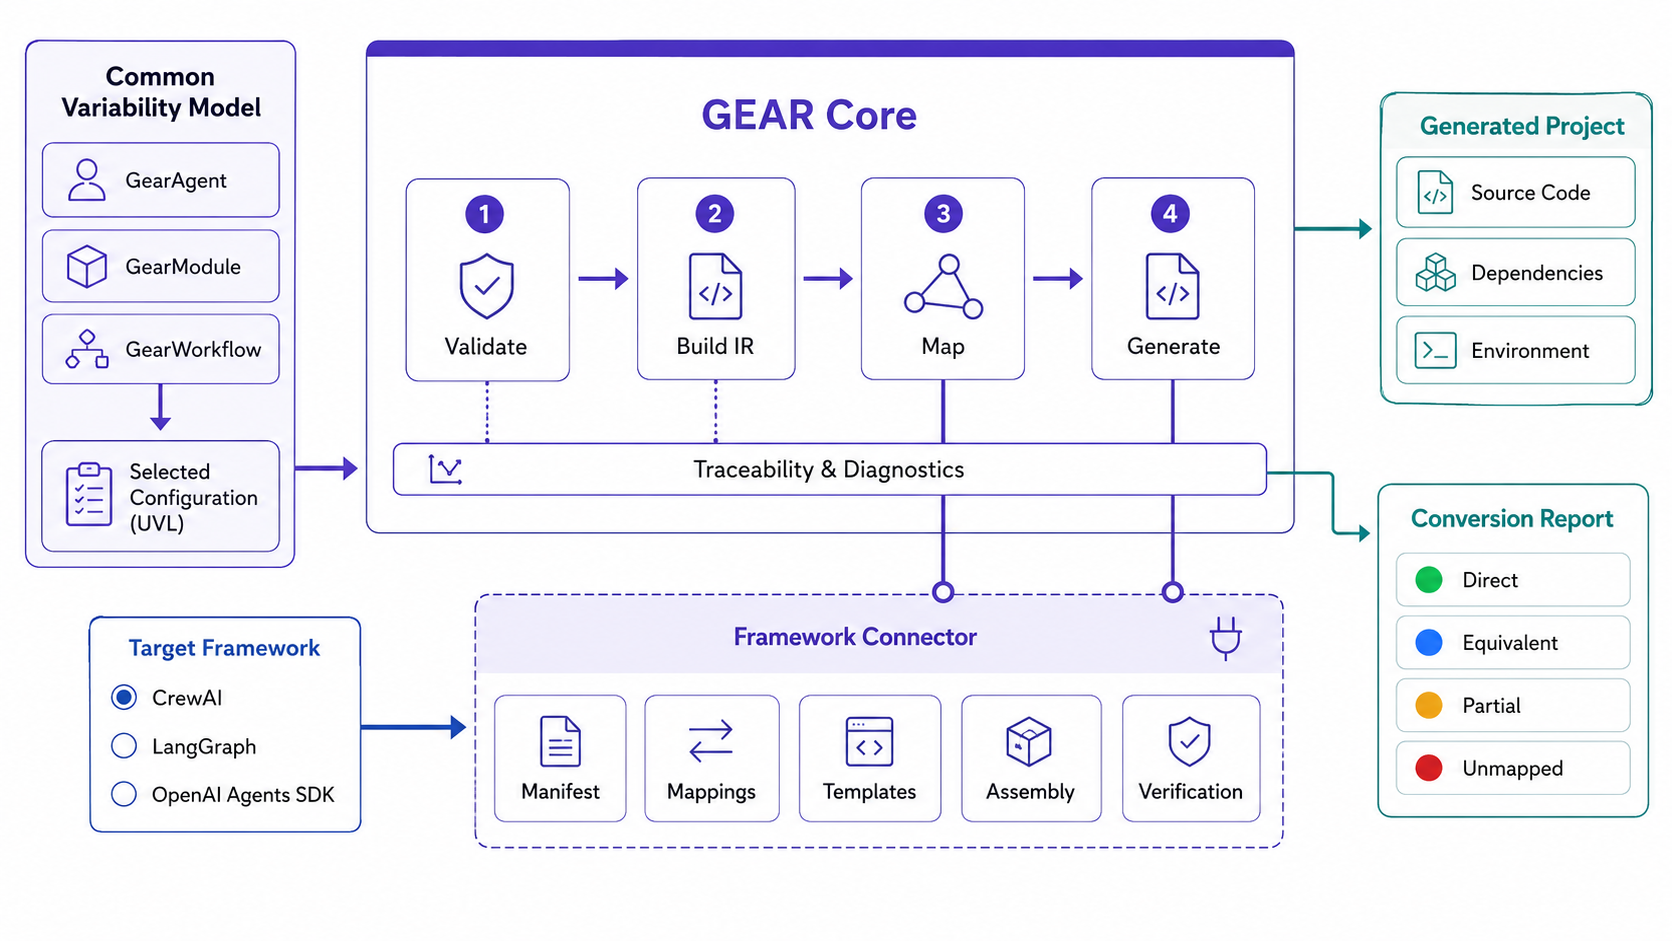
\includegraphics[width=\textwidth]
    {Figures/gear-architecture.png}
    \caption{Architecture and generation workflow of GEAR.}
    \label{fig:gear-architecture}
\end{figure*}


\paragraph{\textbf{Connector organization.}}
Each connector packages the resources required to support a target framework.
Table~\ref{tab:connector-components} summarizes its principal components.

\begin{table*}[t]
    \centering
    \caption{Principal components of a GEAR framework connector.}
    \label{tab:connector-components}
    \footnotesize
    \begin{tabularx}{\textwidth}{
        @{}
        p{0.20\textwidth}
        >{\raggedright\arraybackslash}X
        p{0.27\textwidth}
        @{}
    }
        \toprule
        \textbf{Component}
        & \textbf{Responsibility}
        & \textbf{Produced or consumed information} \\
        \midrule

        Manifest
        & Declares the connector, its target framework, supported artifacts,
        dependencies, and entry points
        & Connector metadata and compatibility information \\

        Mapping files
        & Associate properties of the common representation with
        target-framework abstractions
        & Direct, equivalent, partial, and unmapped correspondences \\

        Templates
        & Define the structure of the generated source files and configuration
        artifacts
        & Source code, dependency files, and environment templates \\

        Assembly plugin
        & Applies framework-specific transformations that cannot be expressed
        through declarative mappings alone
        & Imports, constructors, workflow composition, and execution logic \\

        Verification rules
        & Check target-specific requirements and unsupported combinations
        & Errors, warnings, and compatibility information \\

        \bottomrule
    \end{tabularx}
\end{table*}

The manifest provides the generation core with the information necessary to
load the connector. Mapping files handle correspondences that can be expressed
declaratively. Templates define the structure of the generated artifacts,
whereas the assembly plugin implements transformations that require executable
logic, such as constructing framework objects, connecting graph nodes,
registering tools, or assembling an execution entry point.

This organization avoids embedding framework-specific conditions directly into
the common generation core. A connector may therefore evolve independently when
the API of its target framework changes.


\paragraph{\textbf{Intermediate representation.}}
After validation, GEAR converts the selected features into an intermediate
representation organized around agents, modules, and workflows. Each element
contains its selected properties and references to related elements.

For example, an agent representation may contain its identifier, instructions,
model configuration, task, tools, memory options, and execution controls. A
module representation records its orchestration type, contained elements, and
optional aggregation or stopping configuration. The workflow representation
defines the top-level composition and shared resources.

The intermediate representation also preserves the origin of each property in
the variability model. This traceability allows GEAR to associate generated
elements and conversion diagnostics with the features selected by the user.

\subsection{Configuration Facilities}
\label{subsec:configuration-facilities}

GEAR exposes separate configuration facilities for individual agents, reusable
orchestration modules, and complete workflows. Agent configurations cover
identity, instructions, model parameters, tasks, tools, memory, outputs, and
execution controls. Module configurations capture parallel or iterative
composition, optional aggregation, and stopping conditions. Workflow
configurations assemble agents and modules, declare their dependencies, and
optionally define shared resources.

These facilities are driven by the \texttt{GearAgent},
\texttt{GearModule}, and \texttt{GearWorkflow} feature models. Consequently,
the available choices and their constraints are obtained from the common
variability representation rather than hard-coded for a target framework. The
target selection activates the relevant connector and its compatibility rules
without changing the source configuration.

\subsection{Code Generation and Validation}
\label{subsec:code-generation-validation}

\paragraph{\textbf{Generation workflow.}}
The generation process follows six steps:

\begin{enumerate}
    \item GEAR loads the configurations of the agents, modules, and workflow.

    \item The configurations are validated against their respective feature
    models and cross-tree constraints.

    \item The selected features are normalized into the framework-independent
    intermediate representation.

    \item The mapping files of the selected connector are applied to identify
    the corresponding target abstractions and their level of support.

    \item The connector combines the mapped properties, templates, and assembly
    logic to generate the source code and supporting artifacts.

    \item The generated project and the mapping results are verified before the
    project is returned to the user.
\end{enumerate}

The generated artifacts may include agent definitions, workflow construction
code, an execution entry point, dependency declarations, environment templates,
and framework-specific configuration files. The exact structure depends on the
target connector, while the configured system remains derived from the same
common representation.


\paragraph{\textbf{Verification and conversion report.}}
GEAR performs verification at both the common-model and target-framework
levels. Feature-model validation ensures that the selected configuration
satisfies the structural relations and cross-tree constraints defined in UVL.
Connector-level verification checks whether the mapped values satisfy the
requirements of the target framework.

The result of the conversion is documented in a report that distinguishes
properties mapped directly, represented through an equivalent abstraction,
partially supported, or left unmapped. The report also identifies missing
values, target-specific requirements, and adaptations performed by the
connector.

Consequently, successful code generation does not imply that every selected
property has been translated with identical semantics. The conversion report
makes such differences explicit and prevents partial support from being
presented as complete equivalence.

\subsection{Extending GEAR}
\label{subsec:extending-gear}

Support for a new framework is introduced by creating a connector containing
its manifest, mappings, templates, assembly logic, and verification rules. The
common variability model does not need to be modified when the new framework
provides alternative implementations of concepts already represented by GEAR.

An extension of the common model is required only when the framework introduces
a configuration decision that is relevant beyond its internal API and cannot be
expressed by the existing features. In this case, the new concept must first be
evaluated using the derivation process described in
Section~\ref{subsec:common-variability-model}. Its mappings can then be defined
for the frameworks able to represent it.

This architecture therefore separates three concerns: the definition of the
configuration space through the feature models, the semantic correspondences
expressed through mappings, and the technical generation mechanisms implemented
by the connectors.

\subsection{Implementation and Availability}
\label{subsec:implementation-availability}

GEAR is implemented as an open-source tool whose framework-independent assets
and target-specific assets remain physically separated. The common feature
models are represented in UVL, correspondence rules are stored in YAML mapping
files, and each connector packages its manifest, templates, assembly plugin,
and verification rules. This organization makes the models and mappings
inspectable independently of the generated source code.

The source code, feature models, connectors, and paper artifacts are available
in the public GEAR repository referenced in Section~\ref{data}. The repository
also provides the material required to reproduce the configurations and
framework translations used in this study, while the accompanying demonstration
video illustrates the end-to-end configuration and generation workflow.
